\section{Subshift}

Seja $N \geq 2$. Definimos o conjunto $\Sigma_N$ formado pelas sequências de números naturais limitados entre $1$ e $N$. Precisamente,

$$\Sigma_N = \{ (x_n)_{n=0}^{\infty} \in \NN^{\NN} : 1 \leq x_n \leq N  \textrm{ para todo } n \geq 0 \}.$$

Definimos também a função $d_N : \Sigma_N \times \Sigma_N \to \RR$ que é dada por
$$d_N(x, y) = \sum_{i=0}^\infty \frac{|x_i - y_i|}{N^i},$$
onde $x = (x_n)_{n=0}^{\infty}$ e $y = (y_n)_{n=0}^{\infty}$. Como $\sum_{i=0}^\infty \frac{N-1}{N^i} < \infty$, temos que $d_N$ está bem definida.


\begin{proposition}
$(\Sigma_N, d_N)$ é um espaço métrico.
\end{proposition}


\begin{proof}
Se $x = (x_n)_{n=0}^{\infty}, y = (y_n)_{n=0}^{\infty}, z = (z_n)_{n=0}^{\infty} \in \Sigma_N$, então
\begin{enumerate}
\item $d_N(x, y) \geq 0$, pois $|x_i - y_i| \geq 0$ para todo $i \geq 0$.
\item $d_N(x, y) = d_N(y, x)$, pois $|x_i - y_i| = |y_i - x_i|$ para todo $i \geq 0$.
\item $d_N(x, z) \leq d_N(x, y) + d_N(y, z)$, pois $|x_i - z_i| = |x_i - y_i + y_i - z_i| \leq |x_i - y_i| + |y_i - z_i|$ para todo $i \geq 0$.
\end{enumerate}
Desse modo, $d_N$ é uma distância em $\Sigma_N$ e $(\Sigma_N, d_N)$ é um espaço métrico.
\end{proof}


\begin{proposition}
Sejam $x = (x_n)_{n=0}^{\infty}, y = (y_n)_{n=0}^{\infty} \in \Sigma_N$.
\begin{enumerate}
\item Se $x_i = y_i$ para todo $0 \leq i \leq k$, então $d_N(x, y) \leq \frac{1}{N^k}$.
\item Se $d_N(x, y) < \frac{1}{N^k}$, então $x_i = y_i$ para todo $0 \leq i \leq k$.
\end{enumerate}
\end{proposition}


\begin{proof}
\begin{enumerate}
\item Se $x_i = y_i$ para todo $0 \leq i \leq k$, então
$$d_N(x, y) \leq \sum_{i=k+1}^\infty \frac{N-1}{N^i} = \frac{N-1}{N^{k+1}}\sum_{i=0}^\infty \frac{1}{N^{i}} = \frac{N-1}{N^{k+1}} \frac{N}{N - 1} = \frac{1}{N^k}.$$

\item Se $x_j \neq y_j$ para algum $0 \leq j \leq k$, então
$$d_N(x, y) \geq \frac{1}{N^j} \geq \frac{1}{N^k}.$$
\end{enumerate}
\end{proof}

Definimos a função shift $\sigma: \Sigma_N \to \Sigma_N$ que é dada por $\sigma(x) = (x_n)_{n=1}^\infty$ para todo $x = (x_n)_{n=0}^\infty \in \Sigma_N$, isto é, $\sigma(x_0, x_1, \dots) = (x_1, x_2, \dots)$.

\begin{proposition}
$\sigma$ é contínua.
\end{proposition}

\begin{proof}
Sejam $\varepsilon > 0$ e $x = (x_n)_{n=0}^\infty \in \Sigma_N$. Seja $k \geq 1$ tal que $\frac{1}{N^k} < \varepsilon$ e defina $\delta = \frac{1}{N^{k+1}}$.

Pela Proposição anterior, se $y = (y_n)_{n=0}^\infty \in \Sigma_N$ e $d_N(x, y) < \delta$, então $x_i = y_i$ para todo $i = 0, \dots, k+1$. Desse modo, $\sigma(x)$ e $\sigma(y)$ coincidem nas $k$ primeiras entradas. Utilizando a Proposição anterior novamente, concluímos que $d_N(\sigma(x), \sigma(y)) \leq \frac{1}{N^k} < \varepsilon$.
\end{proof}


Seja $A = (a_{ij})_{1 \leq i,j \leq N}$ uma matriz quadrada de ordem $N$ tal que $a_{ij} \in \{ 0, 1 \}$ para todo $1 \leq i,j \leq N$. Dizemos que $A$ é uma matriz de transição. Definimos o conjunto $\Sigma_A$ como
$$\Sigma_A = \{ (x_n)_{n=0}^{\infty} \in \Sigma_N : a_{x_i x_{i+1}} = 1 \textrm{ para todo } i \geq 0 \}.$$

Seja $x = (x_n)_{n=0}^{\infty} \in \Sigma_A$. Observando que $a_{x_i x_{i+1}} = 1$ para todo $i \geq 1$, temos que $\sigma(x) = (x_n)_{n=1}^\infty \in \Sigma_A$. Desse modo, podemos definir a função $\sigma_A: \Sigma_A \to \Sigma_A$ como sendo a restrição de $\sigma$ em $\Sigma_A$. Dizemos que $\sigma_A$ é o subshift definido por $A$.

\begin{proposition}
$\Sigma_A$ é um subconjunto fechado de $\Sigma_N$.
\end{proposition}


\begin{proof}
Seja $(x_n)_{n=0}^{\infty}$ uma sequência de elementos em $\Sigma_A$ convergente para $x = (\xi_n)_{n=0}^{\infty} \in \Sigma_N$. Observe que a sequência $(x_n)_{n=0}^{\infty}$ é uma sequência de sequências, pois cada $x_n$ é elemento de $\Sigma_N$.

Suponha que $x \notin \Sigma_A$. Então, existe $j \geq 0$ tal que $a_{\xi_j \xi_{j+1}} = 0$. Por outro lado, pela definição de convergência, existe $n_0 \geq 0$ tal que $d(x_{n_0}, x) < \frac{1}{N^{j+1}}$ e, portanto, as $j+2$ primeiras entradas de $x$ e $x_{n_0}$ são iguais. Escrevendo $x_{n_0} = (\eta_n)_{n=0}^\infty$, concluímos que $a_{\eta_j \eta_{j+1}} = a_{\xi_j \xi_{j+1}} = 0$. Absurdo, pois $x_{n_0} \in \Sigma_A$.
\end{proof}


No restante dessa seção vamos estudar a dinâmica da função quadrática $F_\mu(x) = \mu x(1-x)$, onde o parâmetro $\mu = 3.839$ está fixado. Será omitido $\mu$ na notação da função e escreveremos apenas $F$.

Sejam $a = 0.149888$, $\varepsilon = 10^{-3}$ e $I = (a - \varepsilon, a + \varepsilon)$. Através de cálculos é possível mostrar que $F^3(I) \subset I$ e $|(F^3)'(I)| \leq |(F^3)'(a - \varepsilon)| < 1$ e, portanto, o intervalo $I$ possui um ponto periódico atrator de $F$ de período $3$. Se $a_1$, $a_2$ e $a_3$ são os elementos dessa órbita em ordem crescente, então
$$a_1 \simeq 0.149888 \textrm{, } a_2 \simeq 0.489149 \textrm{ e } a_3 \simeq 0.959299.$$
De acordo com o Teorema de Sharkovsky, $F$ possui infinitos pontos periódicos. Além disso, de acordo com o Teorema de Singer, essa é a única órbita atratora de $F$.

De modo análogo, concluímos que $F$ possui outra órbita de tamanho $3$. Se $b_1$, $b_2$ e $b_3$ são os elementos dessa órbita em ordem crescente, então
$$b_1 \simeq 0.169040 \textrm{, } b_2 \simeq 0.539247  \textrm{ e } b_3 \simeq 0.953837.$$

Observando o gráfico de $F^3$, concluímos que para cada $b_i$, existe $b'_i$ no lado oposto de $b_i$ em relação ao ponto $a_i$ tal que $F^3(b'_i) = b_i$. Defina $A_1 = (b'_1, b_1)$, $A_2 = (b'_2, b_2)$ e $A_3 = (b_3, b'_3)$. Cada $A_i$ é exatamente o intervalo maximal contendo $a_i$ utilizado na demonstração do Teorema de Singer.

\begin{center}
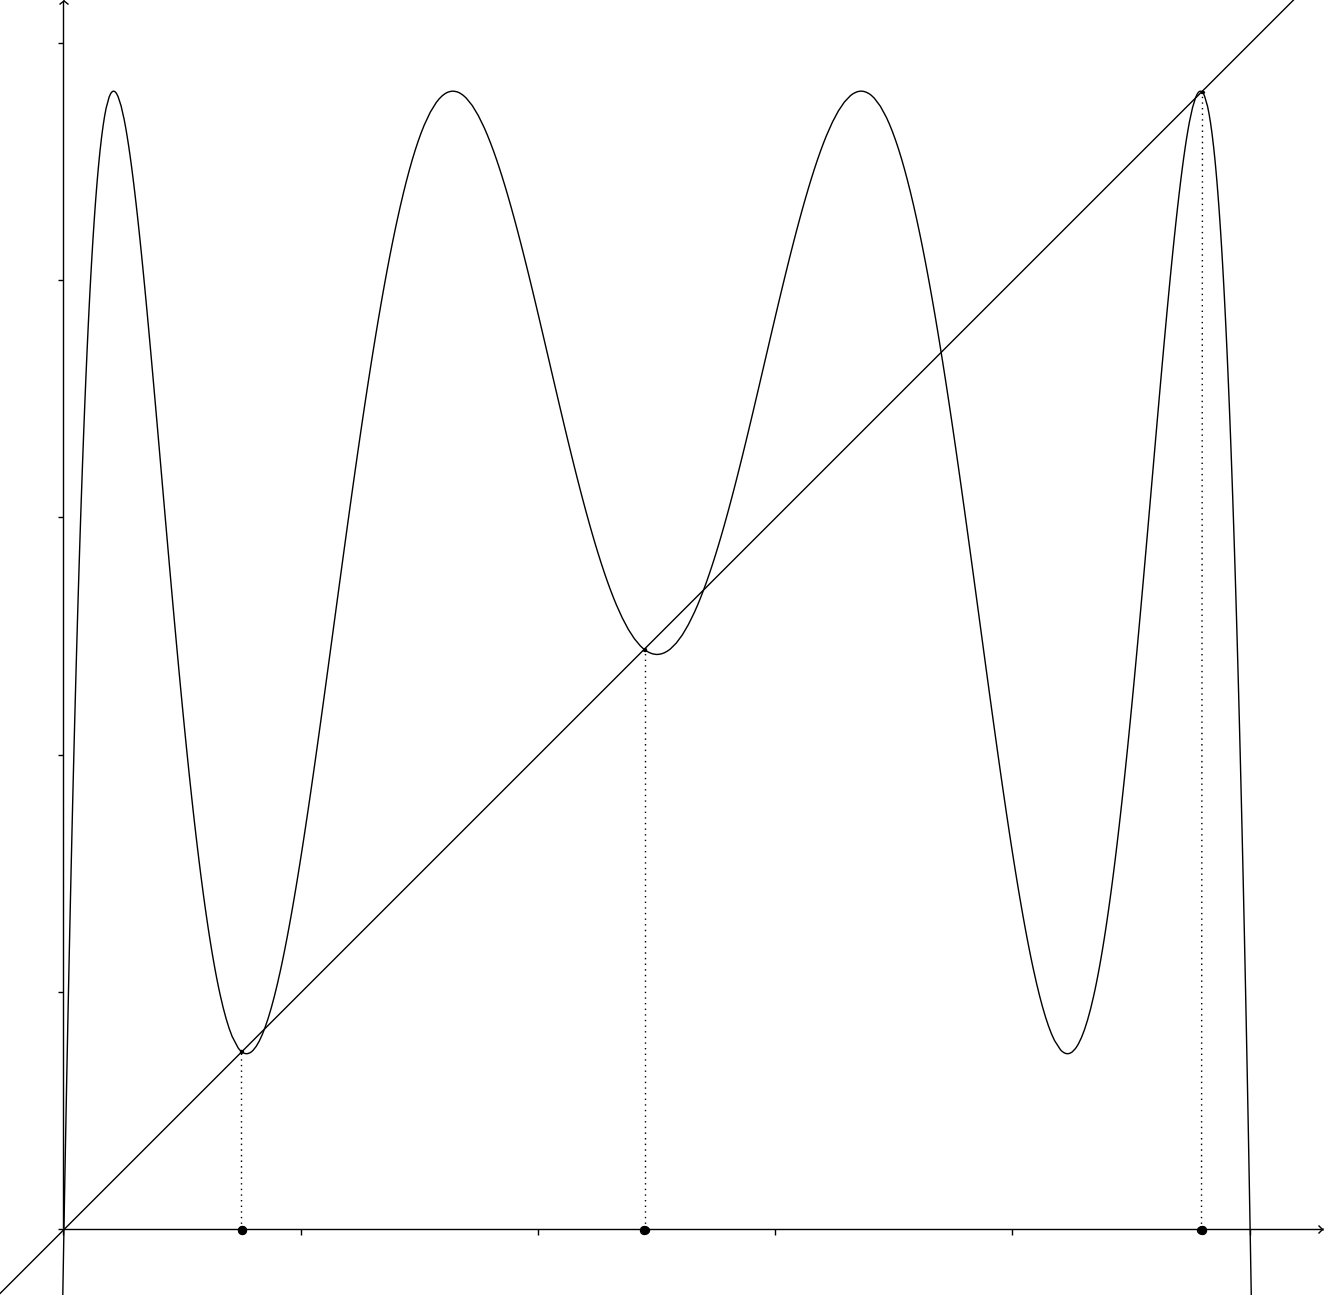
\includegraphics[scale=0.25]{images/f.png}

{\small \textbf{Figura:} Gráfico de $F^3$ com os pontos $a_1$, $a_2$ e $a_3$ assinalados.}
\end{center}

Sendo $F^3$ simétrica em relação ao ponto $\frac{1}{2}$, temos que $F(b'_2) = F(b_2) = b_3$. Além disso, $F(b'_1) = b'_2$ e $F(b'_3) = b'_1$.

\textit{ $\bigstar$ Essas duas últimas igualdades parecem verdadeiras, mas não consegui provar. Ao menos é consistente, pois implica que $b_3' \to b_1' \to b_2' \to b_3 \to b_1 \to b_2$ e, portanto, $F^3(b_i') = b_i$. Tentei mostrar utilizando imagens inversas, mas cada imagem inversa possui dois elementos e eu não consigo construir uma regra sobre qual escolher. $\bigstar$}

Desse modo, $F$ mapeia, de forma monótona, $A_1$ em $A_2$ e $A_3$ em $A_1$. Observando que o máximo de $F$ em $A_2$ é $F \left( \frac{1}{2} \right) = 0.95975 < b'_3$, concluímos que $F(A_2) \subset A_3$.

Sabemos que se $x \notin [0, 1]$, então $\lim_{n \to \infty} F^n(x) = -\infty$. Além disso, o único ponto periódico de $A_i$ é $a_i$ e todos os pontos em $A_i$ tendem para a órbita de $a_i$. Desse modo, todos os outros pontos periódicos de $F$ residem no complemento de $A_1 \cup A_2 \cup A_3$ em $[0, 1]$, que é formado por quatro intervalos fechados. Sejam $I_0 = [0, b'_1]$, $I_1 = [b_1, b'_2]$, $I_2 = [b_2, b_3]$ e $I_3 = [b'_3, 1]$ tais intervalos. A Proposição a seguir nos permite dizer mais.

\begin{proposition}
Se $x \notin \{ 0, a_1, a_2, a_3 \}$ é um ponto periódico de $F$, então $x \in I_1 \cup I_2$.
\end{proposition}


\begin{proof}
Observando que $F$ é monótona em cada $I_k$, temos que $F(I_0) = I_0 \cup A_1 \cup I_1$, $F(I_1) = I_2$, $F(I_2) = I_1 \cup A_2 \cup I_2$ e $F(I_3) = I_0$. Desse modo, se $x \in I_1 \cup I_2$ é periódico, então órbita de $x$ permanece em $I_1 \cup I_2$.

Por outro lado, se $x \in I_0 - \{ 0 \}$, existe um menor $n \geq 1$ tal que $F^n(x) \notin I_0$. Se $F^n(x) \in A_1$, então $x$ não pode ser periódico, pois o único ponto periódico de $A_1$ é $a_1$. Se $F^n(x) \in I_1$, então $x$ não pode ser periódico, pois caso contrário a órbita de $x$ estaria contida em $I_1 \cup I_2$ e nunca retornaria para $I_0$.

Finalmente, se $x \in I_3$, então $F(x) \in I_0$ e a análise segue como no parágrafo anterior.
\end{proof}

Defina o conjunto $\Lambda$ como
$$\Lambda = \{ x \in I_1 \cup I_2 : F^n(x) \in I_1 \cup I_2 \textrm{ para todo } n \geq 1 \}.$$
Pela Proposição anterior, todos os pontos periódicos de $F$ estão em $\Lambda$, com exceção dos pontos $0$, $a_1$, $a_2$ e $a_3$.


\begin{lemma}
Existe $N \geq 1$ tal que $|(F^n)'(\Lambda)| > 1$ para todo $n \geq N$.
\end{lemma}


\begin{proof}
Como $F'' < 0$, temos que $F'$ é estritamente decrescente. Sendo $F'\left(\frac{1}{2}\right) = 0$, concluímos que $A_2$ é uma vizinhança da única raiz de $F'$. Além disso, $|(F^3)'(b_2)| = |(F^3)'(b_2')| \simeq 0.3$. Desse modo, $|F'(I_1 \cup I_2)| \geq \nu$ para algum $\nu \in (0, 1)$.

Observando o gráfico de $F^3$, concluímos que o subconjunto de $I_1 \cup I_2$ no qual $|F'| \leq 1$ é formado por três intervalos fechados. Sejam $B_1$, $B_2$ e $B_3$ tais intervalos, numerados da esquerda para direita. Utilizando a simetria do gráfico de $F^3$ e o fato de que $(F^3)'(b_1) > 1$, temos que $F^3(B_3) \subset A_1$ e, portanto, $B_3 \cap \Lambda = \emptyset$.

Por outro lado, $B_2 \subset [0.661, 0.683]$, já que $(F^3)'(0.661) > 1$ e $(F^3)'(0.683) < -1$. Desse modo, $F(B_2) \subset A_3$. Utilizando novamente a simetria do gráfico de $F^3$, concluímos que $F(B_1) \subset A_3$. Portanto, $B_1 \cap \Lambda = \emptyset$ e $B_2 \cap \Lambda = \emptyset$. Assim, $|(F^3)'(\Lambda)| \geq \lambda$ para algum $\lambda > 1$. Observe que se $x \in \Lambda$ e $L \geq 1$, então
$$\left| \left(F^{3L}\right)'(x) \right| = 
\prod_{i=0}^{L-1} \left| \left( F^3 \right)' \left( F^{3i}(x) \right) \right|
\geq \lambda^L.$$

Finalmente, sejam $x \in \Lambda$ e $K \geq 1$ tal que $\nu^2 \lambda^K > 1$. Se $N = 3K$ e $n \geq N$, podemos escrever $n = 3L + \alpha$, onde $L \geq K$ e $\alpha \in \{ 0, 1, 2 \}$. Desse modo,
\begin{enumerate}
\item[i.] se $\alpha = 0$, então
$$ \left| \left(F^n\right)'(x) \right|
= \left| \left(F^{3L}\right)'(x) \right|
\geq \lambda^L \geq \lambda^K > 1.$$
\item[ii.] se $\alpha = 1$, então
$$ \left| \left(F^n\right)'(x) \right|
= \left| F' \left(F^{3L}(x) \right) \right|
\left| \left(F^{3L}\right)'(x) \right|
\geq \nu \lambda^L > \nu^2 \lambda^K > 1.$$
\item[iii.] se $\alpha = 2$, então
$$ \left| \left(F^n\right)'(x) \right|
= \left| F' \left(F^{3L + 1}(x) \right) \right|
\left| F' \left(F^{3L}(x) \right) \right|
\left| \left(F^{3L}\right)'(x) \right|
\geq \nu^2 \lambda^L \geq \nu^2 \lambda^K > 1.$$
\end{enumerate}


\end{proof}


Para as demonstrações dos próximos resultados, vamos considerar a matriz de transição
$$A = \begin{bmatrix}
0 & 1 \\
1 & 1
\end{bmatrix}.$$
Podemos definir a função $S: \Lambda \to \Sigma_A$ por $S(x) = (x_n)_{n=0}^\infty$, onde $x_i = 1$ se $F^i(x) \in I_1$ e $x_i = 2$ se $F^i(x) \in I_2$ para todo $i \geq 0$. Observe que está $S$ bem definida, pois $F(I_1) = I_2$ e $F(I_2) \subset I_1 \cup I_2$ e, portanto, $a_{x_i x_{i+1}} = 1$ para todo $i \geq 0$. 

\begin{lemma}
$\Lambda$ não contém intervalos.
\end{lemma}

\begin{proof}
Suponha que $\Lambda$ contém algum intervalo e sejam $a, b \in \Lambda$, com $a < b$, tais que $[a, b] \subset \Lambda$. Utilizando a notação do Lema anterior, seja $k \geq N$ tal que $(b - a) \nu^N \lambda^{k - N} > 1$. Pelo Teorema do Valor Médio, existe $c \in [a, b]$ tal que
\begin{align*}
|F^k(b) - F^k(a)| & = |(F^k)'(c)|(b-a) \\
& = \left| \prod_{i=0}^{k-1} F'(F^i(c)) \right| (b-a) \\ 
& = \left| \prod_{i=0}^{N-1} F'(F^i(c)) \right| \left| \prod_{i=N}^{k-1} F'(F^i(c)) \right| (b-a) \\
& \geq \nu^N \lambda^{k-N} (b-a) > 1
\end{align*}
e, portanto, $F^k(a)$ ou $F^k(b)$ não é elemento de $[0,1]$, o que é um absurdo.
\end{proof}

\begin{proposition}
$S$ é um homeomorfismo.
\end{proposition}


\begin{proof}

\begin{enumerate}

\item[i.] $S$ é injetora:

Sejam $x, y \in \Lambda$, com $x < y$, e suponha que $S(x) = S(y)$. Desse modo, $F^n(x)$ e $F^n(y)$ está no mesmo lado em relação ao ponto crítico $\frac{1}{2}$ e, portanto, $F$ é monótona no intervalo $J_n$, cujos pontos extremos são $F^n(x)$ e $F^n(y)$, para todo $n \geq 0$. Desse modo, se $z \in [x, y]$, então $F^n(z) \in J_n \subset I_1 \cup I_2$ para todo $n \geq 0$ e, portanto, $z \in \Lambda$. Mas isso implica que $[x, y] \subset \Lambda$, o que é um absurdo.

\item[ii.] $S$ é sobrejetora:

Seja $(x_n)_{n=0}^\infty \in \Sigma_A$. Vamos provar que existe $x \in \Lambda$ tal que $S(x) = (x_n)_{n=0}^\infty$.

Inicialmente, para cada $n \geq 0$, considere
$$I_{x_0 \cdots x_n} = \{ x \in [0,1] : x \in I_{x_0}, \dots, F^n(x) \in I_{x_n} \}.$$
Observe que $x \in I_{x_0 \cdots x_n}$ se, e somente se, $x \in I_{x_0}$ e $F(x) \in \{ y \in [0,1] : y \in I_{x_1}, \dots, F^{n-1}(y) \in I_{x_n} \}$. Desse modo, $I_{x_0 \cdots x_n} = I_{x_0} \cap F^{-1}(I_{x_1 \cdots x_n})$.

Assim, por indução, é possível concluir que $I_{x_0 \cdots x_n}$ é um intervalo fechado não vazio. Além disso, $I_{x_0 \cdots x_n} = I_{x_0 \cdots x_{n-1}} \cap F^{-n}(I_{x_n}) \subset I_{x_0 \cdots x_{n-1}}$.

Desse modo, $(I_{x_0 \cdots x_n})_{n=0}^\infty$ é uma sequência de intervalos encaixantes fechados e não vazios e, portanto, existe $x \in \cap_{n=0}^\infty I_{x_0 \cdots x_n}$. Como $F^i(x) \in I_{x_i}$ para todo $i \geq 0$, concluímos que $S(x) = (x_n)_{n=0}^\infty$. Observe que $x \in \cap_{n=0}^\infty I_{x_0 \cdots x_n}$ é único, pois $S$ é injetora.

\item[iii.] $S$ é contínua:

Seja $x \in \Lambda$, com $S(x) = (x_n)_{n=0}^\infty$. Sejam também $\varepsilon > 0$ e $k \geq 1$ tal que $\frac{1}{N^k} < \varepsilon$.

Como $I_{x_0 \dots x_k}$ um intervalo fechado e $x \in I_{x_0 \dots x_k}$, tome $\delta > 0$ tal que $y \in \Lambda$ e $|x-y| < \delta$ implica que $y \in I_{x_0 \dots x_k}$. Desse modo, $S(x)$ e $S(y)$ são iguais nas primeiras $k+1$ entradas e, portanto, $d_N(S(x), S(y)) \leq \frac{1}{N^k} < \varepsilon$.

\end{enumerate}
\end{proof}


\begin{theorem}
$S \circ F|_\Lambda = \sigma_A \circ S$.
\end{theorem}


\begin{proof}
Seja $x \in \Lambda$. Utilizando a notação da Proposição anterior, se $S(x) = (x_n)_{n=0}^\infty$, então $x$ é o único elemento de $\cap_{n=0}^\infty I_{x_0 \cdots x_n}$.

Podemos escrever $I_{x_0 \dots x_n} = I_{x_0} \cap F^{-1}(I_{x_1}) \cap \cdots \cap F^{-n}(I_{x_n})$. Se $x_0 = 1$, então $x_1 = 2$ e, portanto, $F(I_{x_0}) = I_{x_1}$. Se $x_0 = 2$, então $F(I_{x_0}) = I_1 \cup A_2 \cup I_2$. Em ambos os casos, $F(I_{x_0}) \supset I_{x_1}$ e, desse modo,
$$F(I_{x_0 \dots x_n}) = I_{x_1} \cap \cdots \cap F^{-n+1}(I_{x_n}).$$
Portanto,
\begin{align*}
S \circ F|_{\Lambda}(x) & = S(F(\cap_{n=0}^\infty I_{x_0 \cdots x_n})) \\
& = S(\cap_{n=1}^\infty I_{x_1 \cdots x_n}) \\
& = (x_n)_{n=1}^\infty  = \sigma \circ S(x)
\end{align*}
\end{proof}


\begin{proposition}
Seja $A$ uma matriz de transição de ordem $N$. Então $\sigma_A$ possui $Tr(A^k)$ pontos periódicos de período $k$.
\end{proposition}


\begin{proof}
Observe que $x = (x_n)_{n=0}^\infty \in \Sigma_N$ é um ponto periódico de período $k$ de $\sigma$ se, e somente se, $x_i = x_{i+k}$ para todo $i \geq 0$, ou seja,
$$x = (x_0, x_1, \dots, x_{k-1}, x_0, x_1, \dots, x_{k-1}, \dots).$$
Desse modo, $x \in \Sigma_A$ se, e somente se, $a_{x_0 x_1} = a_{x_1 x_2} = \cdots = a_{x_{k-1} x_0} = 1$ e, portanto,
\[\begin{cases} 
  a_{x_0 x_1} a_{x_1 x_2}  \dots a_{x_{k-1} x_0} = 1, & \textrm{ se } x \in \Sigma_A \\
  a_{x_0 x_1} a_{x_1 x_2}  \dots a_{x_{k-1} x_0} = 0, & \textrm{ se } x \notin \Sigma_A 
  \end{cases}
\]

Assim, a quantidade de pontos periódicos de período $k$ de $\sigma_A$ é dada por
$$\sum_{1 \leq x_0, \dots, x_{k-1} \leq N} a_{x_0 x_1} a_{x_1 x_2}  \dots a_{x_{k-1} x_0}.$$

Por outro lado, utilizando a definição de multiplicação de matrizes podemos mostrar por indução que $A^k = (c_{ij})_{1 \leq i, j \leq N}$, onde
$$c_{ij} = \sum_{1 \leq x_1, \dots, x_{k-1} \leq N} a_{i x_1} a_{x_1 x_2}  \dots a_{x_{k-1}j}$$
e, portanto,
$$\tr(A^k) = \sum_{x_0 = 1}^N c_{x_0 x_0} = \sum_{1 \leq x_0, \dots, x_{k-1} \leq N} a_{x_0 x_1} a_{x_1 x_2}  \dots a_{x_{k-1} x_0}.$$
\end{proof}











